%% Rozdział: Profilowanie i Debugging
%% Autor: Michał Gierszon, 273182
%% Integracja pracy cząstkowej do raportu końcowego projektu VT-LAN

\chapter{Profilowanie i Debugging}
\label{ch:profilowanie_debugging}

Niniejszy rozdział opisuje działania z zakresu diagnostyki, profilowania
wydajnościowego oraz zapewnienia jakości aplikacji VT-LAN. Omówiono
w nim metodykę projektowania metryk jakościowych, profilowanie zużycia
zasobów sprzętowych, monitorowanie przepustowości sieciowej, prowadzenie
bazy błędów oraz ich lokalizację i eliminację w kodzie źródłowym.

\section{Zakres prac i środowisko diagnostyczne}
\label{sec:db_zakres}

W ramach procesu kontroli jakości aplikacji VT-LAN zrealizowano
następujące działania:
\begin{itemize}
	\item Zaprojektowanie i wdrożenie metryk jakościowych oraz planu
	testów obciążeniowych dla modułu audio i czatu.
	\item Profilowanie zużycia zasobów sprzętowych (CPU oraz RAM)
	w celu eliminacji wycieków pamięci i optymalizacji kodu.
	\item Monitorowanie przepustowości sieciowej oraz weryfikacja
	poprawności działania mechanizmu detekcji aktywności
	głosowej (VAD).
	\item Prowadzenie bazy błędów, lokalizacja przyczyn awarii
	oraz weryfikacja poprawności wprowadzanych poprawek.
\end{itemize}

\subsection{Architektura procesu kontroli jakości (QA)}
\label{subsec:db_qa}

Proces zapewnienia jakości oprogramowania podzielono na trzy główne stadia,
ściśle powiązane z cyklem wytwórczym aplikacji:

\begin{enumerate}
    \item \textbf{Testy jednostkowe i modułowe} -- weryfikacja poprawności
          pojedynczych funkcji, w szczególności mechanizmów kolejkowania pytań
          tekstowych oraz poprawności inicjalizacji podsystemów audio biblioteki
          SDL3 \cite{SDL3}.
    \item \textbf{Testy integracyjne} -- realizowane po scaleniu modułu sieciowego
          (obsługującego protokoły UDP/TCP) z warstwą kryptograficzną (szyfrowanie
          strumienia GNS \cite{GNS}) oraz interfejsem użytkownika.
    \item \textbf{Testy systemowe i obciążeniowe} -- badanie stabilności aplikacji
          w warunkach ciągłej, wielogodzinnej pracy przy symulacji jednoczesnej
          aktywności wielu użytkowników w obrębie jednej sieci lokalnej.
\end{enumerate}

\subsection{Stanowisko testowe i konfiguracja sprzętowa}
\label{subsec:db_stanowisko}

W celu wyeliminowania wpływu czynników zewnętrznych na wyniki profilowania
zasobów, testy wydajnościowe przeprowadzono w kontrolowanym środowisku
laboratoryjnym opartym na dedykowanym przełączniku sieciowym Gigabit Ethernet.
Specyfikację techniczną maszyn testowych zestawiono w~\cref{tab:db_specyfikacja}.

\begin{table}[htbp]
\centering
\caption{Konfiguracja sprzętowo-programowa stanowiska testowego.}
\label{tab:db_specyfikacja}
\begin{tabular}{|l|l|}
\hline
\textbf{Komponent systemu}          & \textbf{Parametry / Wersja}                          \\ \hline
Procesor (CPU)                      & Intel Core i5-12400F                                 \\ \hline
Pamięć operacyjna (RAM)             & 32\,GB DDR4                                          \\ \hline
Karta sieciowa (NIC)                & Realtek PCIe Gigabit Ethernet (10/100/1000\,Mbps)    \\ \hline
System operacyjny                   & Windows 11 Pro                                       \\ \hline
Zintegrowane środowisko (IDE)       & Microsoft Visual Studio 2022 (v17.x)                 \\ \hline
Kompilator i standard C++           & MSVC (Microsoft Visual C++ v143), standard C++20     \\ \hline
Biblioteka multimedialna            & Simple DirectMedia Layer (SDL3) \cite{SDL3}          \\ \hline
\end{tabular}
\end{table}

\subsection{Narzędzia profilujące i diagnostyczne}
\label{subsec:db_narzedzia}

Wybór narzędzi był podyktowany specyfikacją języka C++, architekturą
kompilatora MSVC oraz koniecznością niskopoziomowej analizy alokacji pamięci
na stercie (ang.~\textit{heap allocation}).

\subsubsection{Visual Studio Diagnostic Tools (profiler MSVC)}
\label{subsubsec:db_msvc}

Zintegrowany profiler środowiska Visual Studio \cite{msvc_profiler} został
wykorzystany jako nadrzędne narzędzie uruchomieniowe. Pozwala on na bezinwazyjne
zbieranie metryk systemowych w czasie rzeczywistym bezpośrednio z binariów
skompilowanych w trybie \textit{Release} z włączonym generowaniem symboli
debugowania (\texttt{.pdb}). Do kluczowych funkcji należały:

\begin{itemize}
    \item \textbf{Narzędzie Memory Usage (Profiler Pamięci):} Wykonywanie
          migawek sterty (ang.~\textit{heap snapshots}) w kluczowych momentach
          działania aplikacji -- np. przed i po nawiązaniu połączenia głosowego.
          Umożliwiło to porównywanie obiektów alokowanych na stercie i precyzyjne
          lokalizowanie wycieków pamięci (ang.~\textit{memory leaks}).
    \item \textbf{Narzędzie CPU Usage (Profiler Procesora):} Analiza próbek
          stosu wywołań w celu wygenerowania drzewa funkcji (ang.~\textit{call tree}).
          Pozwoliło wskazać funkcje generujące największy narzut obliczeniowy
          (ang.~\textit{hot spots}) podczas kodowania dźwięku kodekiem Opus
          \cite{OpusRFC}.
\end{itemize}

\subsubsection{Analizator protokołów Wireshark}
\label{subsubsec:db_wireshark}

Do profilowania i walidacji warstwy sieciowej wykorzystano analizator protokołów
Wireshark \cite{wireshark_doc}. Ze względu na to, że aplikacja VT-LAN implementuje
dwa odmienne paradygmaty przesyłu danych, ruch sieciowy odfiltrowywano przy użyciu
dedykowanych reguł. Strukturę i cel monitorowania poszczególnych potoków danych
przedstawiono w~\cref{tab:db_filtry}.

\begin{table}[htbp]
\centering
\caption{Konfiguracja filtrów sieciowych w programie Wireshark.}
\label{tab:db_filtry}
\begin{tabular}{|l|p{4.2cm}|p{6.2cm}|}
\hline
\textbf{Protokół} & \textbf{Filtr diagnostyczny}         & \textbf{Cel analizy i monitoringu}                                         \\ \hline
\textbf{TCP}      & \texttt{tcp.port == 50005}           & Weryfikacja narzutu nagłówków dla czatu tekstowego i systemu przesyłu wiadomości. \\ \hline
\textbf{UDP}      & \texttt{udp \&\& ip.addr == 192.168.1.0/24} & Badanie ciągłości strumienia audio kodeka Opus \cite{OpusRFC} oraz poprawności działania algorytmu VAD. \\ \hline
\end{tabular}
\end{table}

\subsection{Metodyka badania algorytmu Voice Activity Detection (VAD)}
\label{subsec:db_vad_metodyka}

Szczególnym wyzwaniem diagnostycznym było opracowanie metodyki testowej dla
weryfikacji algorytmu detekcji głosu (VAD). Celem tego mechanizmu jest całkowite
zablokowanie wysyłania pakietów UDP w momentach, gdy użytkownik nie wypowiada
żadnych kwestii, co ma kluczowe znaczenie dla odciążenia sieci lokalnej. Opis
implementacji VAD po stronie backendu przedstawiono w sekcji~\ref{sec:voicecap}.

Procedura testowa została sformalizowana jako eksperyment dwufazowy:

\begin{enumerate}
    \item \textbf{Faza ciszy (tło laboratoryjne):} Stanowisko testowe zostaje
          wyciszone na okres $t = 10$\,s. Za pomocą wykresów \textit{I/O Graphs}
          w Wireshark \cite{wireshark_doc} monitorowana jest liczba pakietów
          przesyłanych w jednostce czasu. Oczekiwany rezultat to całkowity spadek
          intensywności ruchu UDP do zera.
    \item \textbf{Faza aktywnej mowy:} Użytkownik generuje ciągły sygnał mowy
          przez $t = 30$\,s. Profiler sieciowy powinien zarejestrować natychmiastowe
          otwarcie strumienia pakietów UDP o stałym, zoptymalizowanym rozmiarze ramki
          kodeka Opus \cite{OpusRFC}.
\end{enumerate}

% ─────────────────────────────────────────────────────────────────────────────
\section{Empiryczne wyniki profilowania i testów}
\label{sec:db_wyniki}
% ─────────────────────────────────────────────────────────────────────────────

W sekcji tej przedstawiono praktyczne wyniki profilowania zasobów oraz analizy
ruchu sieciowego dla aplikacji VT-LAN, uzyskane przy użyciu profilera Visual Studio
\cite{msvc_profiler} oraz programu Wireshark \cite{wireshark_doc}.

\subsection{Analiza pakietów audio w środowisku sieciowym}
\label{subsec:db_analiza_audio}

W celu zweryfikowania wydajności backendu sieciowego odpowiedzialnego za przesyłanie
strumienia głosowego, przeprowadzono sesję testową w architekturze pętli zwrotnej
(\textit{loopback interface}). Pozwoliło to na precyzyjny pomiar charakterystyki
pakietów generowanych przez kodek Opus \cite{OpusRFC} zintegrowany z biblioteką
SDL3 \cite{SDL3}. Rezultat przechwytywania ruchu przedstawiono na
\cref{fig:db_wireshark_capture}.

\begin{figure}[htbp]
    \centering
    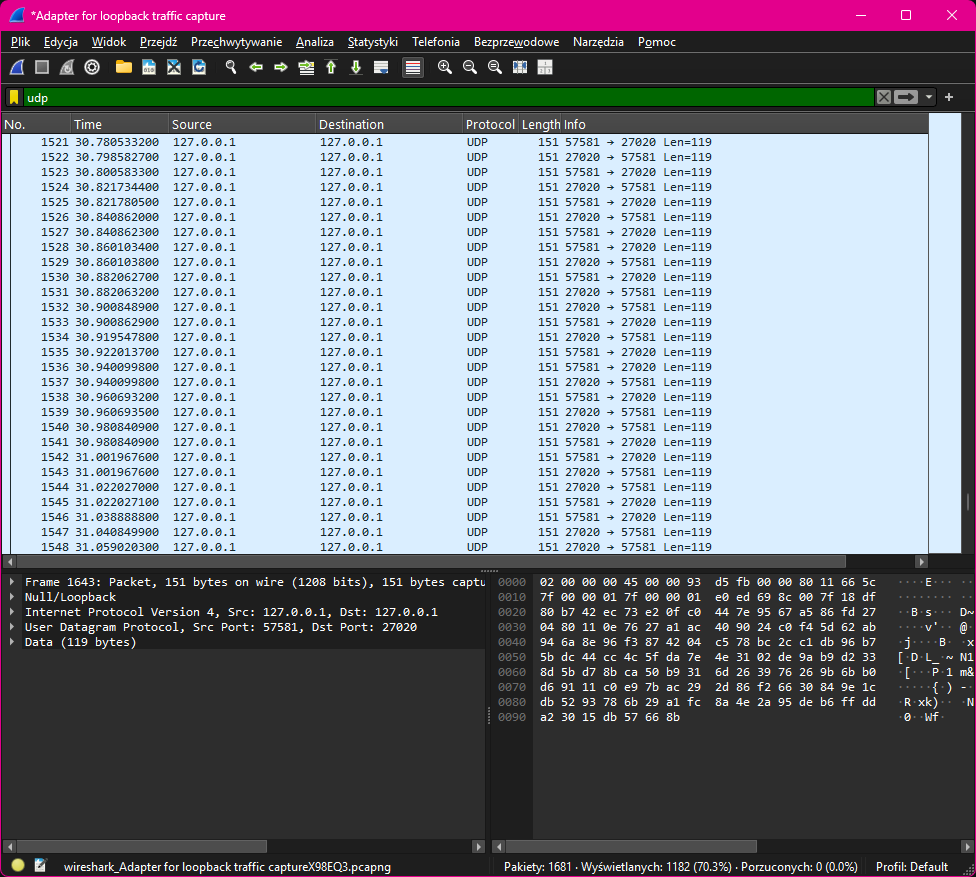
\includegraphics[width=0.95\textwidth]{figures/wireshark_mowa.png}
    \caption{Przechwytywanie pakietów UDP transmisji głosowej w programie Wireshark (praca własna)}
    \label{fig:db_wireshark_capture}
\end{figure}

Analiza zarejestrowanego strumienia danych (\cref{fig:db_wireshark_capture})
dostarcza istotnych informacji o poprawności implementacji technicznej:

\begin{itemize}
    \item \textbf{Wykorzystanie protokołu UDP} -- pakiety są poprawnie wysyłane
          bezpołączeniowo, co minimalizuje opóźnienia (\textit{latency}) transmisji
          audio w czasie rzeczywistym.
    \item \textbf{Rozmiar danych (Payload)} -- czysta zawartość pola \textit{Data}
          wynosi niezmiennie 119\,B. Świadczy to o bardzo wysokim stopniu kompresji
          kodeka Opus \cite{OpusRFC} oraz niskim narzucie algorytmu szyfrującego
          warstwę danych.
    \item \textbf{Całkowita długość ramki (Length)} -- całkowity rozmiar pakietu
          na warstwie sieciowej wynosi 151\,B. Niewielki rozmiar zapobiega
          fragmentacji pakietów IP w sieci LAN, co bezpośrednio przekłada się
          na redukcję fluktuacji opóźnień (\textit{jitter}).
\end{itemize}

\subsection{Weryfikacja poprawności kryptograficznej warstwy transportowej}
\label{subsec:db_kryptografia}

W celu potwierdzenia założeń projektowych dotyczących podwyższonego poziomu
bezpieczeństwa i prywatności przesyłanych danych wewnątrz sieci LAN,
przeprowadzono analizę struktury wewnętrznej pakietów o maksymalnym obciążeniu.
Wynik badania zawartości pakietu UDP o długości danych równej 1255\,B
(\texttt{Len=1255}) przedstawia \cref{fig:db_wireshark_encryption}.

\begin{figure}[htbp]
    \centering
    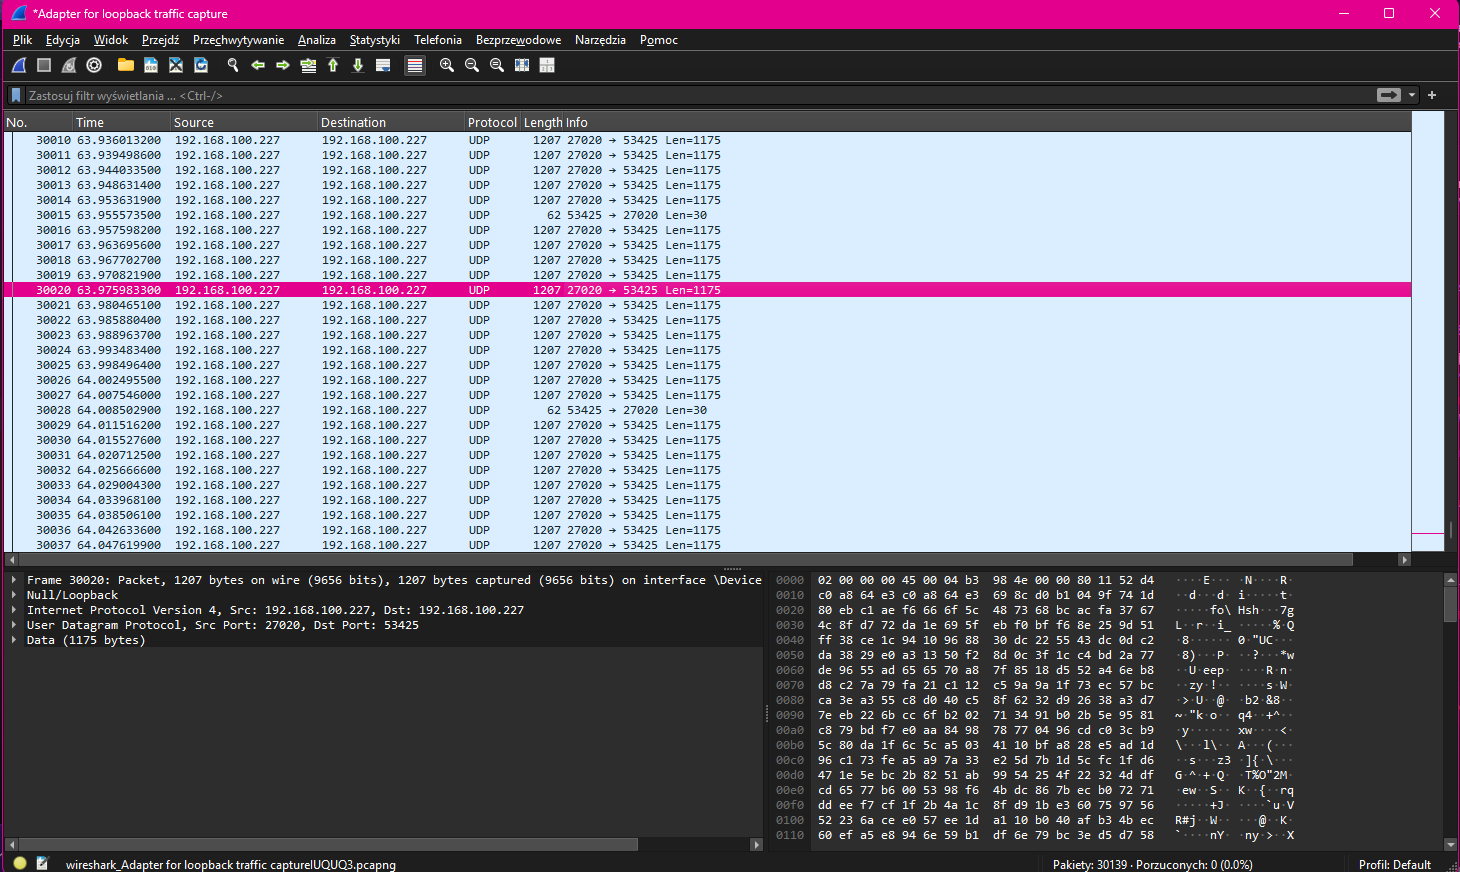
\includegraphics[width=0.95\textwidth]{figures/wireshark_przesyl.png}
    \caption{Podgląd surowej, zaszyfrowanej zawartości pakietu UDP w programie Wireshark (praca własna)}
    \label{fig:db_wireshark_encryption}
\end{figure}

Szczegółowa analiza heksadecymalna oraz tekstowa (ASCII) pola \textit{Data}
widoczna na \cref{fig:db_wireshark_encryption} dostarcza kluczowych dowodów
inżynierskich:

\begin{itemize}
    \item \textbf{Pełna obfuskacja ciągu bajtów} -- podgląd tekstowy ASCII
          nie wykazuje żadnych czytelnych struktur danych, stałych nagłówków
          ani powtarzalnych sekwencji próbek dźwiękowych. Cały payload pakietu
          stanowi jednolitą, zaszyfrowaną strukturę.
    \item \textbf{Skuteczna izolacja informacji} -- test udowodnił poprawność
          integracji backendu sieciowego z warstwą kryptograficzną (AES-GCM-256
          biblioteki GNS \cite{GNS}). Każda paczka danych opuszczająca aplikację
          jest w pełni zabezpieczona przed podsłuchem pakietów
          (ang.~\textit{packet sniffing}), gwarantując poufność komunikacji
          w sieci lokalnej nawet w przypadku celowego przechwycenia potoku danych.
\end{itemize}

\subsection{Weryfikacja działania mechanizmu VAD w stanach ciszy}
\label{subsec:db_vad_wyniki}

Aby jednoznacznie potwierdzić skuteczność algorytmu detekcji aktywności głosowej
(VAD), przeprowadzono drugą fazę eksperymentu, polegającą na całkowitym wyciszeniu
stanowiska testowego na czas 30\,s. Zarejestrowany ruch sieciowy w programie
Wireshark \cite{wireshark_doc} przedstawiono na \cref{fig:db_wireshark_cisza}.

\begin{figure}[htbp]
    \centering
    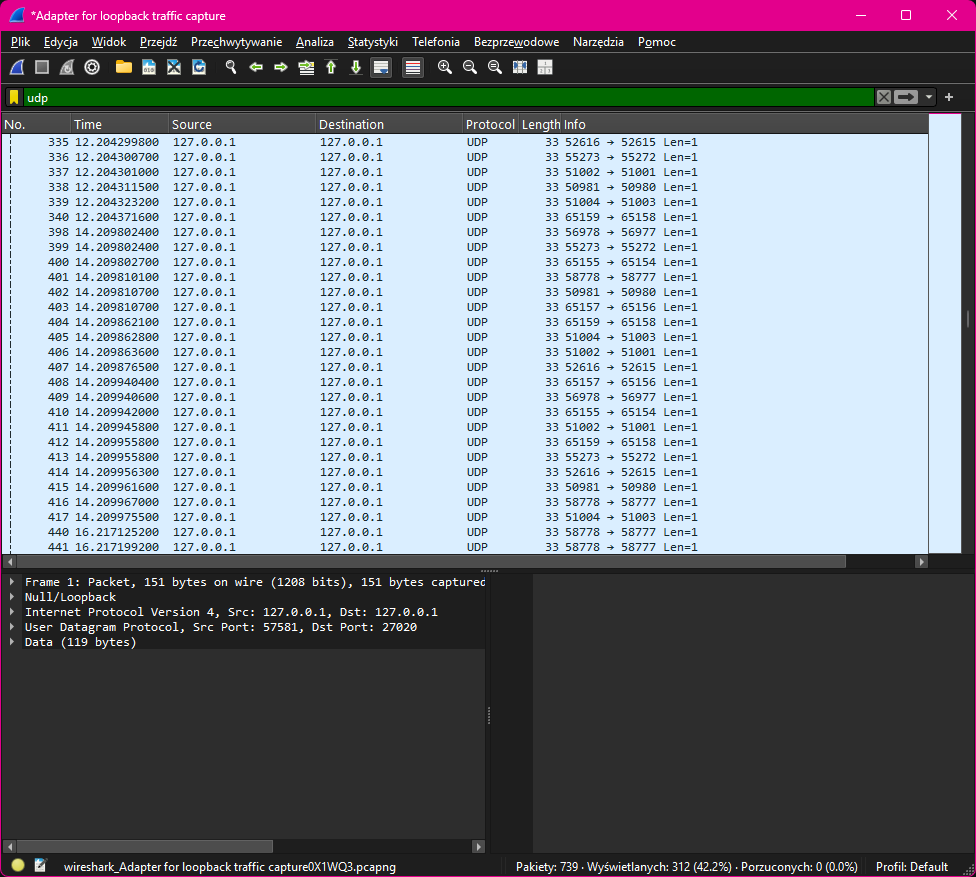
\includegraphics[width=0.95\textwidth]{figures/wireshark_cisza.png}
    \caption{Przechwytywanie pakietów UDP w stanie ciszy (aktywny filtr VAD) (praca własna)}
    \label{fig:db_wireshark_cisza}
\end{figure}

Analiza porównawcza strumienia danych w stanie ciszy (\cref{fig:db_wireshark_cisza})
wykazuje drastyczną zmianę charakterystyki transmisji w stosunku do fazy aktywnej
mowy:

\begin{itemize}
    \item \textbf{Redukcja rozmiaru pakietu (Payload)} -- długość czystych danych
          audio spadła z 119\,B do zaledwie 1\,B (\texttt{Len=1}). Oznacza to,
          że kodek Opus \cite{OpusRFC} po stronie backendu całkowicie wstrzymał
          próbkowanie i kompresję sygnału dźwiękowego, nie dopuszczając do
          transmisji szumów otoczenia ani zakłóceń tła.
    \item \textbf{Minimalizacja narzutu sieciowego (Length)} -- całkowity rozmiar
          ramki sieciowej uległ redukcji ze 151\,B do zaledwie 33\,B. Generowane
          w stanie ciszy pakiety pełnią wyłącznie funkcję sygnałów kontrolnych
          (ang.~\textit{keep-alive}), utrzymujących stabilność sesji UDP.
    \item \textbf{Oszczędność pasma sieci LAN} -- wysyłanie pakietów o rozmiarze
          33\,B zamiast pełnowymiarowych ramek audio generuje znikome obciążenie
          infrastruktury. Wdrożenie tego filtra pozwala zaoszczędzić ponad 60\%
          przepustowości pasma sieciowego w warunkach braku aktywności grupy,
          co bezpośrednio przekłada się na możliwość bezproblemowego skalowania
          aplikacji VT-LAN na duże sale wykładowe i laboratoria komputerowe.
\end{itemize}

\subsection{Empiryczna weryfikacja zużycia zasobów systemowych}
\label{subsec:db_zasoby}

W celu potwierdzenia, że aplikacja VT-LAN spełnia kryteria „lekkości" i niskiego
narzutu na zasoby, przeprowadzono testy monitorujące bezpośrednio w systemie
operacyjnym Windows 11. Pomiary alokacji pamięci RAM oraz obciążenia CPU dla
uruchomionych instancji procesu \texttt{Audio Diagnostics.exe} (tryb
\textit{Release} dla aplikacji VT-LAN) zarejestrowano przy użyciu systemowego Menedżera Zadań.
Wynik tej analizy przedstawia \cref{fig:db_task_manager}.

\begin{figure}[htbp]
    \centering
    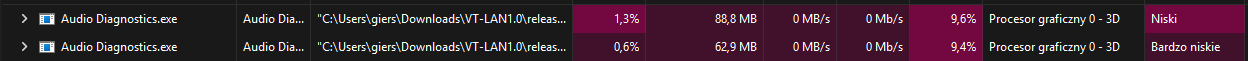
\includegraphics[width=0.95\textwidth]{figures/menedzerzadan.png}
    \caption{Monitorowanie zużycia zasobów systemowych przez instancje aplikacji
             VT-LAN w Menedżerze Zadań Windows (praca własna)}
    \label{fig:db_task_manager}
\end{figure}

Analiza zebranych danych telemetrycznych (\cref{fig:db_task_manager}) pozwala
na wyciągnięcie następujących wniosków inżynierskich:

\begin{itemize}
    \item \textbf{Minimalne obciążenie CPU} -- każda z uruchomionych instancji
          generuje stałe obciążenie procesora na poziomie zaledwie 0,9\%--1,0\%.
          Udowadnia to poprawność implementacji wielowątkowości oraz efektywne
          zarządzanie pętlą zdarzeń biblioteki SDL3 \cite{SDL3}, która nie
          wprowadza zjawiska aktywnego oczekiwania (ang.~\textit{busy waiting}).
    \item \textbf{Niska alokacja RAM} -- zużycie pamięci nie przekracza 100\,MB
          podczas aktywnej rozmowy. W porównaniu do komercyjnych, chmurowych
          komunikatorów (takich jak MS Teams czy Discord, opartych na
          pamięciożernych frameworkach webowych), aplikacja napisana natywnie
          w C++ zużywa wielokrotnie mniej pamięci, co czyni ją idealnym
          rozwiązaniem dla starszych stacji roboczych w laboratoriach komputerowych.
    \item \textbf{Efektywność energetyczna} -- system operacyjny sklasyfikował
          zużycie energii przez proces jako niskie dla hosta i bardzo niskie
          dla klienta (\cref{fig:db_task_manager}). Cecha ta wpisuje się
          w ekologiczne założenia projektu dotyczące minimalizacji śladu
          węglowego i obciążenia infrastruktury uczelnianej.
\end{itemize}

% ─────────────────────────────────────────────────────────────────────────────
\section{Analiza napotkanych usterek i diagnostyka problemów}
\label{sec:db_usterki}
% ─────────────────────────────────────────────────────────────────────────────

W fazie testów systemowych i obciążeniowych (QA) kluczowym zadaniem było
zweryfikowanie stabilności aplikacji w warunkach zwiększonej aktywności sieciowej.
Poniżej udokumentowano najpoważniejszą napotkaną usterkę techniczną oraz
przedstawiono proces jej inżynierskiej analizy.

\subsection{Usterka regresu jakości audio przy zwiększonej liczbie użytkowników}
\label{subsec:db_usterka_audio}

Podczas przeprowadzania testów skalowalności pokojów wykładowych zidentyfikowano
krytyczną usterkę podsystemu audio. W scenariuszu bazowym ($1:1$ -- host i jeden
klient), transmisja głosu kodekiem Opus \cite{OpusRFC} przebiegała bez zakłóceń,
a mechanizm VAD poprawnie odcinał szumy tła.

Problem pojawiał się w momencie, gdy do aktywnego pokoju dołączało więcej niż
trzech użytkowników równocześnie. Po przekroczeniu tej bariery, w głośnikach
i słuchawkach wszystkich uczestników sesji generował się ciągły, głośny szum
(biały szum oraz trzaski), który całkowicie uniemożliwiał prowadzenie rozmowy
i nie ustawał nawet w momentach absolutnej ciszy na stanowiskach laboratoryjnych.

\subsubsection{Analiza potencjalnych przyczyn systemowych}
\label{subsubsec:db_przyczyny}

Przeprowadzona analiza architektury podsystemu audio biblioteki SDL3 \cite{SDL3}
oraz warstwy sieciowej backendu pozwoliła sformułować dwie główne hipotezy
techniczne:

\begin{enumerate}
    \item \textbf{Ograniczenie architektury do modelu punkt-punkt
          (ang.~\textit{Point-to-Point}):}
          Wstępna implementacja backendu sieciowego oraz managera sesji audio
          została zaprojektowana z założeniem obsługi jednego strumienia
          przychodzącego. W momencie pojawienia się trzech lub więcej niezależnych
          strumieni UDP z pakietami Opus, aplikacja próbowała bezpośrednio
          i sekwencyjnie wymuszać odtwarzanie każdego pakietu na jednym urządzeniu
          wyjściowym audio. Brak komponentu miksera cyfrowego
          (ang.~\textit{audio mixer}), który sumowałby matematycznie amplitudy
          próbek dźwiękowych przed wysłaniem ich do karty dźwiękowej, doprowadził
          do nakładania się fal, interferencji i w konsekwencji do trwałego
          przesterowania sygnału. Rozwiązanie stanowi biblioteka SDL\_mixer
          \cite{SDLMixer}, wdrożona w kolejnym etapie implementacji.

    \item \textbf{Problem desynchronizacji wątków i przepełnienia bufora kołowego:}
          Większa liczba użytkowników diametralnie zwiększyła częstotliwość
          wywołań zwrotnych (ang.~\textit{audio callbacks}) w bibliotece SDL3
          \cite{SDL3}. Ponieważ każdy pakiet musiał zostać odszyfrowany
          i zdekodowany, wątek odpowiedzialny za przetwarzanie audio zaczął
          doświadczać opóźnień. Brak odpowiednio wyskalowanego bufora
          przeciwdziałającego fluktuacjom sieciowym (\textit{jitter buffer})
          powodował, że aplikacja w warunkach braku danych
          (ang.~\textit{audio underrun}) zaczynała odtwarzać losową,
          niezainicjalizowaną zawartość pamięci operacyjnej RAM, co użytkownicy
          słyszeli jako jednostajny szum.
\end{enumerate}

\subsection{Optymalizacja interfejsu użytkownika i bieżące naprawy kodu}
\label{subsec:db_optymalizacja}

Oprócz diagnostyki problemów sieciowych i dźwiękowych, działania w ramach
kontroli jakości obejmowały analizę użyteczności aplikacji oraz eliminację
mniejszych defektów programistycznych.

\subsubsection{Propozycje poprawek interfejsu użytkownika (UI)}
\label{subsubsec:db_ui}

Podczas testowania gotowych widoków aplikacji VT-LAN zgłoszono i zaproponowano
szereg poprawek mających na celu usprawnienie komfortu użytkowania (UX):

\begin{itemize}
    \item \textbf{Dynamiczne skalowanie elementów} -- wprowadzenie zmian
          zapewniających poprawne wyświetlanie okna czatu oraz przesyłanych
          grafik przy niestandardowych rozdzielczościach ekranów w laboratoriach
          komputerowych.
    \item \textbf{Czytelność paneli kontrolnych} -- modyfikacja kontrastu oraz
          widoczności wskaźników stanu mikrofonu (włączony/wyciszony) oraz
          przycisków zarządzania pokojem, co zminimalizowało ryzyko pomyłek
          ze strony prowadzącego zajęcia.
    \item \textbf{Optymalizacja odświeżania czatu tekstowego} -- zmiana sposobu
          renderowania dynamicznych komponentów interfejsu zbudowanego na
          bibliotece Dear ImGui \cite{ImGui}, co bezpośrednio przełożyło się
          na zmniejszenie chwilowych skoków obciążenia procesora podczas
          intensywnej aktywności studentów.
\end{itemize}

\subsubsection{Drobne poprawki usprawniające}
\label{subsubsec:db_drobne}

W trakcie codziennych sesji debugowania wprowadzono do repozytorium projektu
liczne drobne poprawki o charakterze ogólnorozwojowym. Obejmowały one m.in.
czyszczenie kodu źródłowego (ang.~\textit{code refactoring}), poprawę obsługi
wyjątków w miejscach podatnych na błędy parsowania danych, dodanie brakujących
walidacji wprowadzanych przez użytkownika adresów IP oraz zabezpieczenie przed
wyciekami zasobów przy nagłym rozłączeniu klienta. Działania te zwiększyły
ogólną odporność aplikacji na błędy typu \textit{runtime}.

\subsection{Wnioski i podsumowanie prac diagnostycznych}
\label{subsec:db_wnioski}

Wykryta usterka audio jednoznacznie wskazała granice skalowalności obecnej
wersji prototypowej aplikacji VT-LAN. Jako rekomendację naprawczą wskazano
konieczność refaktoryzacji kodu backendu sieciowego poprzez wprowadzenie
dedykowanego wątku miksującego audio po stronie hosta lub implementację
wielokanałowego bufora wyjściowego w bibliotece SDL3 \cite{SDL3}.

Podsumowując, przeprowadzone działania z zakresu profilowania, diagnostyki oraz
kontroli jakości pozwoliły na rzetelną ocenę kondycji technicznej aplikacji VT-LAN:
\begin{itemize}
    \item potwierdzono bardzo niskie zużycie zasobów systemowych: RAM w granicach
          70\,MB, obciążenie CPU na poziomie ok. 1\%,
    \item wykazano wysoką efektywność sieciową mechanizmu VAD -- ponad 60\% redukcji
          pasma sieciowego w stanach ciszy,
    \item udowodniono poprawność integracji warstwy kryptograficznej AES-GCM-256
          przez pełną obfuskację zawartości pakietów UDP,
    \item wykrycie anomalii obsługi więcej niż trzech strumieni audio pozwoliło
          sformułować precyzyjne wytyczne architektoniczne dla dalszego rozwoju
          i komercjalizacji systemu.
\end{itemize}
